\documentclass{article}
\usepackage{tikz}
\usepackage[utf8]{inputenc}
\usepackage[pdftex]{hyperref} 
\usepackage{xcolor}
\usetikzlibrary{decorations.pathreplacing}
\usepackage{indentfirst}
\usepackage[cache=false]{minted}
\usepackage{graphicx}

\graphicspath{./}

\definecolor{light-gray}{gray}{0.95}
\newcommand{\code}[1]{\colorbox{light-gray}{\texttt{#1}}}

\hypersetup{
    colorlinks=true,
    linkcolor=blue,
    urlcolor=blue,
}

\setminted[json]{
    numbersep=5pt,
    autogobble,
    frame=lines,
    framesep=2mm,
    fontsize=\footnotesize,
    style=emacs
}
\setminted[md]{
    numbersep=5pt,
    autogobble,
    frame=lines,
    framesep=2mm,
    fontsize=\footnotesize,
    style=emacs
}


\title{\textbf{Projet de programmation}}
\date{Jan 2022 - Avr 2022}
\author{Nahaki Barry \and Mathias Crema \and Maxime Dumonteil \and Nicolas Hubner \and Maxime Meyrat \and Alex Pepi}

\begin{document}

\maketitle
\newpage

\renewcommand{\contentsname}{Sommaire}
\tableofcontents
\cleardoublepage
 
\newpage
 
\renewcommand{\listfigurename}{Liste des figures}
\listoffigures
 
\newpage

\section{Présentation du projet}
Le but de ce projet est de créer un programme capable de jouer à des jeux d'enchères. La difficulté de ces jeux est qu'ils sont à information partielle et sont basés sur des probabilités pour maximiser le gain final. Nous avons décidé de nous focaliser sur le jeu Blackjack.

\subsection{Présentation du jeu}

Les sources utilisées pour la rédaction de cette partie ont été deux guides de Blackjack de sites spécialisés \cite{blackjack_regles_1} \cite{blackjack_regles_2}.

\subsubsection{Le Blackjack : un jeu de carte}

Le Blackjack est un jeu d'enchère qui utilise un jeu de carte classique de 52 cartes. Le paquet de carte comporte donc 4 couleurs (Coeur, Carreau, Pique, Trèfle) et pour chaque couleur il y a un As, des cartes numérotées de 2 à 10, un Valet, une Dame et un Roi.

\subsubsection{Les acteurs}

Les deux acteurs de ce jeu sont :
\begin{itemize}
    \item \textbf{La banque (le croupier)} qui distribue les cartes et joue "contre" les joueurs.
    \item \textbf{Les joueurs} qui misent et ceux-ci gagnent ou perdent en fonction de leurs cartes et des règles du jeu.
\end{itemize}

\subsubsection{Les règles du jeu en détail}

Tout d'abord, précisons que nous allons nous baser sur les règles officielles du Blackjack (appliquées dans les casinos aux États-Unis) et nous ne nous intéresserons pas aux différentes variantes qui peuvent exister comme le "Blackjack 6:5" ou encore le "Blackjack Royal Match".

\bigskip

Voici donc les règles officielles du Blackjack :

\begin{itemize}
    \item \textbf{Le nombre de joueur} \newline
    Une partie de Blackjack se joue avec un croupier et entre 1 et 7 joueurs.

    \item \textbf{Le but du jeu} \newline
    Chaque joueur a comme but d'atteindre 21 points avec ses cartes, sans le dépasser, ou battre le croupier.\\
    Un joueur bat le croupier lorsqu'il a plus de points que lui ou que le croupier dépasse 21 points.\\
    Un joueur perd lorsqu'il dépasse 21 points ou a moins de points que le croupier.\\
    Lorsqu'un joueur perd, il perd sa mise initiale, sinon, il la gagne avec un ratio dépendant de son score (explication ci-dessous).

    \item \textbf{Déroulement d'une partie}
    \begin{enumerate}
        \item Chaque joueur mise une somme d'argent.
        \item Le croupier distribue une carte face visible à chaque joueur ainsi que lui-même. Il distribue ensuite une deuxième carte face visible à chaque joueur et se distribue une carte face cachée.
        \item Chaque joueur joue leur tour de jeu.
        \item Le croupier joue son tour.
        \item On calcule les scores et les mises perdues/gagnées pour chaque joueur.
    \end{enumerate}
    
    
    \item \textbf{Un tour de joueur} \newline
    Un tour de joueur est composé de plusieurs actions. Son tour s'arrête lorsqu'il décide d'arrêter ou qu'il n'a plus le droit de faire des actions.\\
    Les différentes actions possibles sont :
    \begin{itemize}
        \item Demander une carte supplémentaire
        \item S'arrêter de jouer
        \item Doubler sa mise et recevoir une carte. Après cette action, le tour du joueur est terminé.
        \item Abandonner : il perd alors la moitié de sa mise
        \item \textbf{Cas spécial qui ne sera pas appliqué dans notre application : Le split} : Si le joueur a la même carte en double (ex : 2 valets).
    \end{itemize}
    Un joueur n'a plus le droit de faire d'actions après s'être arrêté de jouer, abandonner, doubler, ou perdre.
    
    \item \textbf{Un tour du croupier} \newline
    Le croupier tire des cartes tant qu'il a 16 points ou moins. Il s'arrête s'il a 17 points ou plus.

    \item \textbf{La valeur des cartes} 
    \begin{itemize}
        \item L'As : sa valeur peut être choisie, 1 ou 11.
        \item Les cartes numérotées (2, 3, 4, 5, 6, 7, 8, 9, 10) : valeur égale à la numérotation de la carte.
        \item Les figures (Valet, Dame, Roi) : valeur égale à 10.
    \end{itemize}

    \item \textbf{Décompte des scores} \newline
    Lorsque chaque joueur et le croupier ont fini leur tour, la partie est terminée et le décompte des scores est alors réalisé.
    Le score d'un joueur est la somme des valeurs de ses cartes.
    Si un joueur a 21 points avec seulement deux cartes, on dit qu'il a un \textit{blackjack}.
    
    Voici ci-dessous un résumé précis et concis du décompte des scores trouvable sur la page Wikipédia française de Blackjack : 

    \begin{itemize}\itshape
        \item \textbf{Les joueurs perdants} : Les joueurs ayant plus de 21 points perdent l'intégralité de leurs mises.

        \item \textbf{Les joueurs qui ont un blackjack :}
        Les joueurs récupéreront alors leurs mises. Si le croupier n'a pas de blackjack les joueurs gagnent en plus 1.5 fois leurs mises.
        
        \item \textbf{Les joueurs qui ont 21 points ou moins sans blackjack} 
        \begin{itemize}\itshape
            \item \textbf{Si le croupier a plus de 21 points} alors les joueurs récupèrent leurs mises de départ et gagnent en plus une fois leurs mises.
            \item \textbf{Si le croupier a 21 points ou moins (sans blackjack) :}
                \begin{itemize}
                \item Les joueurs ayant moins de points que le croupier perdent leurs mises.
                \item Les joueurs ayant autant de points que le croupier récupèrent leurs mises.
                \item Les joueurs ayant plus de points que le croupier récupèrent leurs mises et gagnent une fois leurs mises.
                \end{itemize}
        \end{itemize}
    \end{itemize}
\end{itemize}
\bigskip

\subsection{Le logiciel à développer}

Le logiciel final se décompose en plusieurs sections distinctes : 
\begin{itemize}
    \item Un joueur du jeu. Un joueur donnera au moteur son action à chaque tour de jeu. Il peut être humain comme IA.
    \item Le moteur de jeu. Il sera responsable d'exécuter une partie de Blackjack entre plusieurs joueurs et de l'afficher.
    \item Le lanceur de moteur de jeu. Il sera responsable de créer le moteur et de le paramétrer correctement en fonction de ce que l'utilisateur du logiciel demandera.
\end{itemize}

Le moteur est un objet qui a un ensemble de joueur sur lesquels il peut demander l'action à jouer en fonction de l'état du jeu. Le moteur ne connaît pas (et n'a pas à connaître) comment le joueur va "réfléchir", c'est l'implémentation du joueur qui dictera sa réflexion.

Cela permet de pouvoir changer très facilement de type de joueur. Il peut ainsi y avoir un joueur qui "réfléchit" en lisant sur l'entrée standard, ou en calculant grâce à une IA.

De plus, le moteur et son affichage seront dissociés afin de pouvoir passer d'une interface textuelle à une interface graphique facilement.

\bigskip

Le lanceur de moteur de jeu permet de demander à l'utilisateur du logiciel comment il veut lancer une partie, c'est-à-dire combien de joueur, quels types de joueurs, etc. L'utilisateur rentrera ces paramètres avec des arguments de la ligne de commande, ou dans un fichier de paramètres. (voir les besoins pour plus d'informations)

\bigskip

Le logiciel fournira le lanceur de moteur de jeu, le moteur de jeu, ainsi que deux implémentations de joueur par défaut, un joueur "humain", et un joueur "IA" (voir leurs besoins respectifs).

\bigskip

\subsubsection{Résumé d'exécution du logiciel}

\bigskip

\begin{figure}[h!]
    \centering
    
    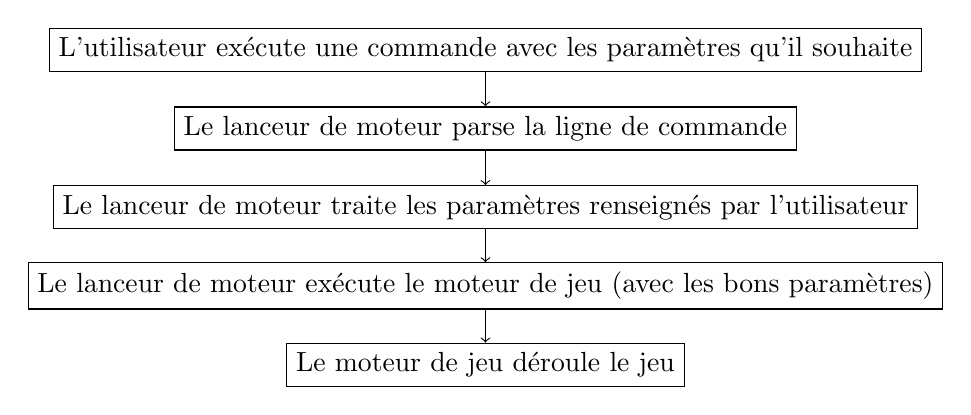
\begin{tikzpicture}
        \node[draw] (user) at (0,0) {L'utilisateur exécute une commande avec les paramètres qu'il souhaite};
        \node[draw] (parse) at (0,-1) {Le lanceur de moteur parse la ligne de commande};
        \node[draw] (param) at (0,-2) {Le lanceur de moteur traite les paramètres renseignés par l'utilisateur};
        \node[draw] (option) at (0,-3) {Le lanceur de moteur exécute le moteur de jeu (avec les bons paramètres)};
        \node[draw] (start) at (0,-4) {Le moteur de jeu déroule le jeu};
        
        \draw[->] (user) -- (parse);
        \draw[->] (parse) -- (param);
        \draw[->] (param) -- (option);
        \draw[->] (option) -- (start);
    \end{tikzpicture}
    
    \caption{Diagramme d'exécution logiciel}
    \label{fig:diag_exec}
    \vspace{0.5cm}Diagramme résumant les étapes techniques du lancement du logiciel. 
\end{figure}

\newpage

\subsubsection{Résumé du déroulement d'une partie (par le moteur de jeu)}

\bigskip

\begin{figure}[h!]
    \centerline{
        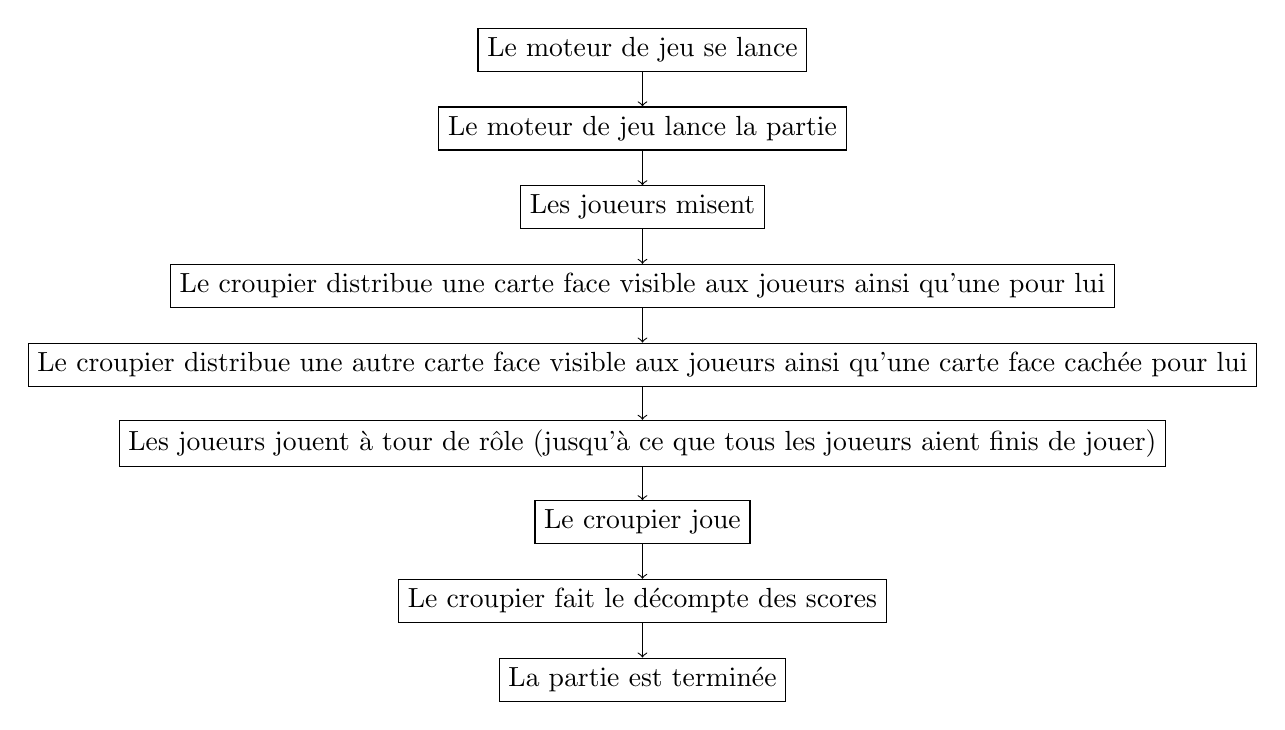
\begin{tikzpicture}[]
            \node[draw] (start1) at (0,0) {Le moteur de jeu se lance};
            \node[draw] (start2) at (0,-1) {Le moteur de jeu lance la partie};
            \node[draw] (bet) at (0,-2) {Les joueurs misent};
            \node[draw] (distrib1) at (0,-3) {Le croupier distribue une carte face visible aux joueurs ainsi qu'une pour lui};
            \node[draw] (distrib2) at (0,-4) {Le croupier distribue une autre carte face visible aux joueurs ainsi qu'une carte face cachée pour lui};
            \node[draw] (play1) at (0,-5) {Les joueurs jouent à tour de rôle (jusqu'à ce que tous les joueurs aient finis de jouer)};
            \node[draw] (play2) at (0,-6) {Le croupier joue};
            \node[draw] (score) at (0,-7) {Le croupier fait le décompte des scores};
            \node[draw] (end) at (0,-8) {La partie est terminée};
            
            \draw[->] (start1) -- (start2);
            \draw[->] (start2) -- (bet);
            \draw[->] (bet) -- (distrib1);
            \draw[->] (distrib1) -- (distrib2);
            \draw[->] (distrib2) -- (play1);
            \draw[->] (play1) -- (play2);
            \draw[->] (play2) -- (score);
            \draw[->] (score) -- (end);
        \end{tikzpicture}
    }

    \caption{Diagramme de déroulement d'une partie}
    \label{fig:diag_partie}
    \vspace{0.5cm}Diagramme résumant les étapes très général d'un déroulement d'une seule partie avec x joueurs.
\end{figure}

\section{Analyse de l'existant}
Il existe de nombreuses Intelligences Artificielles capables de jouer à des jeux d'enchères qui se basent sur des informations partielles, mais surtout pour le Poker. Celles-ci peuvent être très intéressantes et sont capables de battre les meilleurs joueurs du monde dans certains cas comme les intelligences artificielles Deepstack \cite{deepstack} ou Libratus \cite{libratusBlog}.

Dans notre cas, nous nous intéressons aux IA pouvant jouer au Blackjack. Tout d’abord, il faut prendre en compte l'existence de multiples stratégies que l’on peut bien sur appliquer via un ordinateur, des plus basiques \cite{stratBasique} à des versions basées sur les probabilités \cite{blackjack_statistics} \cite{stratProba} afin d’obtenir par exemple les meilleurs gains possibles durant la partie. Précisons aussi qu’il a été décelé des stratégies improductives, que nous pouvons donc éviter dans le comportement de notre IA \cite{stratNull}.
Pour les algorithmes d’IA jouant au Blackjack, il y a peu de programmes accessibles (surtout comparé à ceux réservés au Poker). Néanmoins il existe des projets proches de ce que l’on cherche comme un programme permettant de générer une base de données de mains de joueur possibles (en fonction des paramètres de la partie) \cite{gitBJDataset}, ou encore des IA s’appuyant sur des méthodes de deep ou machine learning \cite{gitBJmachineLearning}. Ces dernières sont bien plus avancées que les précédentes car en termes de temps de calcul et de réussite elles sont plus performantes  \cite{blogBJmachineLearning}. 

Néanmoins la visibilité des algorithmes liés aux jeux d’argent (et particulièrement au Blackjack) reste très limitée car il est question d’argent donc n’est pas accessible au public.
C’est pourquoi il est difficile pour nous de se baser sur un projet existant réellement convaincant et correspondant à ce que nous voulons, c’est-à-dire des intelligences artificielles qui jouent au Blackjack.


\section{Description des besoins}

Les besoins fonctionnels sont ordonnés par ordre de priorité. En fonction de leur importance, ils sont notés de 1 à 3 (1 étant le niveau avec le plus de priorité). La priorité des besoins est déterminée par rapport à ce que nous jugeons être le plus important dans l'application. \\

Pour certains besoins, nous allons évoquer une machine de spécification minimale, c'est à dire, un ordinateur pouvant exécuter l'application avec des composants de puissance minimale. Une machine de spécification minimale doit donc être pourvue à minima de 4Go de mémoire vive, d'un simple processeur basique (exemple : dual core 1.7Ghz), de 50Mo d'espace de stockage et ne nécessite pas de GPU.

\subsection{Besoins fonctionnels}

\subsubsection{Le lanceur de moteur de jeu}

\begin{enumerate}

    \item \textbf{Analyser les arguments de la ligne de commande :}\\
    Pour connaître les paramètres de la partie, le programme du lanceur de moteur de jeu analyse les arguments et enregistre les valeurs données. Si le nom de l'argument n'est pas reconnu, il est ignoré (ainsi que sa valeur). Une valeur associée à un argument doit avoir une taille inférieure à 100 caractères. Si la valeur d'un argument n'est pas correcte, le lanceur doit annoncer l'erreur et arrêter le logiciel. L'utilisateur, joueur ou non de la partie de jeu qui va suivre, décide de la valeur des arguments à fournir (ceci est alors valable et applicable pour les besoins qui suivent concernant les arguments de la ligne de commande). \\
    \textbf{Priorité :} 1. \\
    \textbf{Risques :}
    \begin{itemize}
        \item aucun argument n'est reconnu par le logiciel.
        \item un argument attend une valeur d'un type de données précis mais un autre est renseigné.
        \item un argument est trop long en nombre de caractères.
        \item un argument demandant une valeur mais sans valeur spécifiée.
        \item un argument obligatoire n'est pas renseigné.
    \end{itemize}
    \textbf{Parade :} Afficher un message d'erreur, spécifiant le type d'erreur rencontré. \\
    \textbf{Tests :}
    \begin{itemize}
        \item \textbf{Données :} une machine de spécification minimale, l'application développée, une ligne de commande.
        \item \textbf{Résultats attendus :} positif: l'application lancée correctement, négatif: un message d'erreur.
        \item \textbf{Scénario positif :}
        \begin{itemize}
            \item L’utilisateur ouvre un terminal.
            \item L’utilisateur entre une commande avec des arguments valides.
            \item L'application se lance correctement en prenant en compte les arguments.
        \end{itemize}
        \item \textbf{Scénario négatif :}
        \begin{itemize}
            \item L’utilisateur ouvre un terminal.
            \item L’utilisateur entre une commande avec des arguments invalides.
            \item Un message d'erreur apparaît.
        \end{itemize}
    \end{itemize}
    
    \item \textbf{Sélectionner le type de joueur (humain/IA) :} \\
    L'argument \code{--joueurs} permet de donner le type ainsi que le nombre des joueurs participants. Les valeurs de ce paramètre peuvent être exprimées par ce regex \code{(<type> <nombre>? )+}. Si il n'y a pas de nombre fourni avec le type, la valeur par défaut, 1 (un), est choisie comme quantité. Une partie peut être lancée uniquement avec des joueurs IA, uniquement des joueurs humains ou les deux.
    Les types possibles sont \code{humain} (pour un joueur humain), \code{ia-basique} (pour une ia appliquant une stratégie basique) et \code{ia-hilo} (pour une ia appliquant une stratégie Hi-Lo). \\
    \textbf{Priorité :} 1. \\
    \textbf{Risques :}
    \begin{itemize}
        \item un type autre que \code{humain}, \code{ia-basique} ou \code{ia-hilo} est donné.
        \item un nombre négatif est donné.
        \item le nombre total de joueur (humain + IA) est supérieur à 7.
    \end{itemize}
    \textbf{Parade :} Afficher un message d'erreur, spécifiant le type d'erreur rencontré.\\
    \textbf{Tests :}
    \begin{itemize}
        \item \textbf{Données :} une machine de spécification minimale, l'application développée, une ligne de commande.
        \item \textbf{Résultats attendus :} positif: l'application correctement lancée, négatif: un message d'erreur.
        \item \textbf{Scénario positif:}
        \begin{itemize}
            \item L’utilisateur ouvre un terminal.
            \item L’utilisateur entre la commande avec l'argument \code{--joueurs (ia 5? )+}.
            \item L'application se lance correctement avec 5 joueurs IA.
        \end{itemize}
        \item \textbf{Scénario négatif:}
        \begin{itemize}
            \item L’utilisateur ouvre un terminal.
            \item L’utilisateur entre la commande avec l'argument \code{--joueurs (humain 16? )+}.
            \item Un message d'erreur apparaît.
        \end{itemize}
    \end{itemize}

    \item \textbf{Lancer un ensemble de parties de jeu :} \\
    Le paramètre \code{--parties <nombre>} permet de définir le nombre de parties que le logiciel va lancer. Le nombre de partie de Blackjack doit être compris entre 0 et 500 inclus.
    Un joueur n'a pas le droit de partir entre plusieurs parties (si le programme est lancé pour 10 parties, chaque joueur devra jouer les 10 parties). Dans le cas où cet argument n'est pas renseigné, le logiciel lancera une seule et unique partie, après laquelle le programme s'arrêtera. Les parties sont lancées consécutivement. Chaque partie se déroule selon les règles du blackjack et les valeurs des arguments passées dans la ligne de commande au départ. \\
    \textbf{Priorité :} 2. \\
    \textbf{Risques :}
    \begin{itemize}
        \item une valeur négative est donnée.
        \item une valeur supérieure à 500 est donnée.
    \end{itemize}
    \textbf{Parade :} Afficher un message d'erreur, spécifiant le type d'erreur rencontré.\\
    \textbf{Tests :}
    \begin{itemize}
        \item \textbf{Données :} une machine de spécification minimale, l'application développée, une ligne de commande.
        \item \textbf{Résultats attendus :} positif: l'application correctement lancée, négatif: un message d'erreur.
        \item \textbf{Scénario positif :}
        \begin{itemize}
            \item L’utilisateur ouvre un terminal.
            \item L’utilisateur entre la commande avec l'argument \code{--parties 25}.
            \item L'application se lance correctement et va exécuter 25 parties.
        \end{itemize}
        \item \textbf{Scénario négatif :}
        \begin{itemize}
            \item L’utilisateur ouvre un terminal.
            \item L’utilisateur entre la commande avec l'argument \code{--parties -7}.
            \item Un message d'erreur apparaît.
        \end{itemize}
    \end{itemize}
    
    \item \textbf{Sélectionner la quantité d'argent de départ par joueur:}\\
    L'argument \code{--argent}, avec comme valeur une liste de nombre détermine la somme d'argent que les joueurs ont au départ de l'exécution. L'ordre de ces nombres correspond à l'ordre des joueurs déterminé par \code{--joueurs}.
    Par exemple \code{--joueurs humain 1 ia 2 --argent 10 20 10} se traduit par un joueur humain avec 10 jetons, un joueur IA avec 20 jetons et un joueur IA avec 10 jetons. La somme d'argent de départ d'un joueur doit être comprise entre 0 et 100 000 inclus. \\
    \textbf{Priorité :} 2. \\
    \textbf{Risques :}
    \begin{itemize}
        \item une valeur inférieure à 5 est donnée.
        \item une valeur supérieure à 100 000 est donnée.
        \item le nombre de valeur ne correspond pas au nombre de joueur.
    \end{itemize}
    \textbf{Parade :} Afficher un message d'erreur, spécifiant le type d'erreur rencontré.\\
    \textbf{Tests :}
    \begin{itemize}
        \item \textbf{Données :} une machine de spécification minimale, l'application développée, une ligne de commande.
        \item \textbf{Résultats attendus :} positif: l'application correctement lancée, négatif: un message d'erreur.
        \item \textbf{Scénario positif :}
        \begin{itemize}
            \item L’utilisateur ouvre un terminal.
            \item L’utilisateur entre la commande avec l'argument \code{--argent 4000 500 6000}.
            \item L'application se lance correctement avec les sommes spécifiées.
        \end{itemize}
        \item \textbf{Scénario négatif :}
        \begin{itemize}
            \item L’utilisateur ouvre un terminal.
            \item L’utilisateur entre la commande avec l'argument \code{--argent 9999999 3 6000}.
            \item Un message d'erreur apparaît.
        \end{itemize}
    \end{itemize}

    \item \textbf{Sélectionner le nombre de paquet de cartes à utiliser:}\\
    L'option \code{--paquets} détermine le nombre de paquet de cartes que le moteur utilisera durant le jeu. Le nombre de paquet doit être compris entre 1 et 7 inclus. Si il n'y a pas de nombre précisé, la valeur par défaut est 1. \\
    \textbf{Priorité :} 2. \\
    \textbf{Risques :}
    \begin{itemize}
        \item une valeur inférieure à 1 est donnée.
        \item une valeur supérieure à 7 est donnée.
    \end{itemize}
    \textbf{Parade :} Afficher un message d'erreur, spécifiant le type d'erreur rencontré.\\
    \textbf{Tests :}
    \begin{itemize}
        \item \textbf{Données :} une machine de spécification minimale, l'application développée, une ligne de commande.
        \item \textbf{Résultats attendus :} positif: l'application correctement lancée, négatif: un message d'erreur.
        \item \textbf{Scénario positif :}
        \begin{itemize}
            \item L’utilisateur ouvre un terminal.
            \item L’utilisateur entre la commande avec l'argument \code{--paquets 3}.
            \item L'application se lance et prépare 3 paquets de cartes.
        \end{itemize}
        \item \textbf{Scénario négatif :}
        \begin{itemize}
            \item L’utilisateur ouvre un terminal.
            \item L’utilisateur entre la commande avec l'argument \code{--paquets 8}.
            \item Un message d'erreur apparaît.
        \end{itemize}
    \end{itemize}
    
    \vspace{1cm}
    \begin{figure}[h!]
        \includegraphics[width=\textwidth]{ {files/Diagramme_renouvellement_paquet.png}}
        \caption{Schéma de renouvellement des paquets}
        \label{fig:diag_use_min_bet}
        \vspace{0.5cm} Schéma mettant en scène l'utilisation des multiples paquets et leur renouvellement à chaque début de partie.
    \end{figure}
    \vspace{0.5cm}
    
    \item \textbf{Afficher les statistique d'exécution de l'ensemble des parties :} \\
    Après avoir lancé toutes les parties de Blackjack, le logiciel affiche les statistiques de ces parties de jeu (voir le moteur pour les statistiques affichées). \\
    \textbf{Priorité :} 2. \\
    \textbf{Risques :} aucun. \\
    \textbf{Parade :} aucune.

    \item \textbf{Lire les paramètres du lanceur de moteur de jeu via un fichier:}\\
    Le fichier sera donné via l'argument \code{--fichier params.json}. Si cet argument existe, aucun autre argument n'est pris en compte dans la ligne de commande. C'est le fichier qui dicte les paramètres. Le format des données du fichier est JSON. Voir l'annexe pour un exemple du format utilisé. \\
    \textbf{Priorité :} 3. \\
    \textbf{Risques :}
    \begin{itemize}
        \item le format du fichier ne correspond pas à un \code{.json}.
        \item le fichier est corrompu.
        \item les valeurs du fichier ne correspondent pas à des arguments.
        \item les arguments spécifiés ne sont pas complets.
    \end{itemize}
    \textbf{Parade :} Afficher un message d'erreur, spécifiant le type d'erreur rencontré.\\
    \textbf{Tests :}
    \begin{itemize}
        \item \textbf{Données :} une machine de spécification minimale, l'application développée, une ligne de commande, un fichier JSON, un fichier HTML.
        \item \textbf{Résultats attendus :} positif: l'application correctement lancée, négatif: un message d'erreur.
        \item \textbf{Scénario positif :}
        \begin{itemize}
            \item L’utilisateur ouvre un terminal.
            \item L’utilisateur entre la commande avec l'argument \code{--fichier params.json}.
            \item L'application se lance correctement et récupère bien les arguments depuis le fichier JSON.
        \end{itemize}
        \item \textbf{Scénario négatif :}
        \begin{itemize}
            \item L’utilisateur ouvre un terminal.
            \item L’utilisateur entre la commande avec l'argument \code{--fichier params.html}.
            \item Un message d'erreur apparaît.
        \end{itemize}
    \end{itemize}

    \item \textbf{Sélectionner la mise minimum:}\\
    L'argument \code{--mise-min} détermine la mise minimum par joueur. Cet argument est optionnel. Si il n'est pas renseigné alors la mise minimum de défaut de 5 (cinq) jetons est utilisée. La valeur de mise doit être comprise entre 5 et 100 000 inclus. \\
    \textbf{Priorité :} 3. \\
    \textbf{Risques :}
    \begin{itemize}
        \item une valeur inférieure à 5 est donnée.
        \item une valeur supérieure à 100 000 est donnée.
    \end{itemize}
    \textbf{Parade :} Afficher un message d'erreur, spécifiant le type d'erreur rencontré.\\
    \textbf{Tests :}
    \begin{itemize}
        \item \textbf{Données :} une machine de spécification minimale, l'application développée, une ligne de commande.
        \item \textbf{Résultats attendus :} positif: l'application correctement lancée, négatif: un message d'erreur.
        \item \textbf{Scénario positif :}
        \begin{itemize}
            \item L’utilisateur ouvre un terminal.
            \item L’utilisateur entre la commande \code{--mise-min 20}.
            \item L'application se lance correctement avec une mise minimale de 20 jetons.
        \end{itemize}
        \item \textbf{Scénario négatif :}
        \begin{itemize}
            \item L’utilisateur ouvre un terminal.
            \item L’utilisateur entre la commande \code{--mise-min 3}.
            \item Un message d'erreur apparaît.
        \end{itemize}
    \end{itemize}
    
    \vspace{1cm}
    \begin{figure}[h!]
        \includegraphics[width=\textwidth]{ {files/Diagramme_utilisation_miseMin.png} }
        \caption{Schéma d'utilisation de la mise minimal}
        \label{fig:diag_use_min_bet}
        \vspace{0.5cm} Schéma mettant en scène l'utilisation de la mise minimale par le moteur de jeu pour l'intégration d'un joueur à une partie.
    \end{figure}
    
    \item \textbf{Sélectionner la mise maximum:}\\
    L'argument \code{--mise-max} détermine la mise maximum par joueur. Cet argument est optionnel. Si il n'est pas renseigné alors il n'y a pas de mise maximum (dans la limite où le joueur peut miser une telle quantité). La valeur de mise doit être comprise entre 5 et 100 000 inclus. \\
    \textbf{Priorité :} 3. \\
    \textbf{Risques :}
    \begin{itemize}
        \item une valeur inférieure à 5 est donnée.
        \item une valeur supérieure à 100 000 est donnée.
    \end{itemize}
    \textbf{Parade :} Afficher un message d'erreur, spécifiant le type d'erreur rencontré.\\
    \textbf{Tests :}
    \begin{itemize}
        \item \textbf{Données :} une machine de spécification minimale, l'application développée, une ligne de commande.
        \item \textbf{Résultats attendus :} positif: l'application correctement lancée, négatif: un message d'erreur.
        \item \textbf{Scénario positif :}
        \begin{itemize}
            \item L’utilisateur ouvre un terminal.
            \item L’utilisateur entre la commande \code{--mise-max 1000}.
            \item L'application se lance correctement avec une mise maximale de 1 000 jetons.
        \end{itemize}
        \item \textbf{Scénario négatif :}
        \begin{itemize}
            \item L’utilisateur ouvre un terminal.
            \item L’utilisateur entre la commande \code{--mise-max 2}.
            \item Un message d'erreur apparaît.
        \end{itemize}
    \end{itemize}

    \item \textbf{Afficher un récapitulatif des paramètres:} \\
    Avant l'exécution des parties, le lanceur de moteur de jeu affichera les paramètres renseignés afin que l'utilisateur puisse voir les paramètres d'exécution. \\
    \textbf{Priorité :} 3. \\
    \textbf{Risques :} aucun. \\
    \textbf{Parade :} aucune.

    \item \textbf{Lancer le programme en exécution rapide:} \\
    Lorsqu'il n'y a que des IA qui jouent, le paramètre \code{--rapide} permet de n'afficher que les résultats de chaque partie (et pas le détail de chaque tour). L'intérêt est de pouvoir exécuter beaucoup de parties rapidement et sans affichage superflu car, par exemple, on souhaite tester l'IA ou observer uniquement la finalité de chaque partie de Blackjack.
    Lorsque cet argument est utilisé alors qu'il y a des joueurs humains il n'a pas d'effet et est ignoré.\\
    \textbf{Priorité :} 3. \\
    \textbf{Risques :} aucun. \\
    \textbf{Parade :} aucune.
 
    \item \textbf{Permettre d'utiliser des raccourcis d'argument:} \\ 
    Chaque argument du logiciel devra avoir une version courte. Par exemple \code{--paquets} aura comme version courte \code{-p}. \\
    \textbf{Priorité :} 3. \\
    \textbf{Risques :} aucun. \\
    \textbf{Parade :} aucune.

\end{enumerate}


\subsubsection{Le moteur de jeu}

\begin{enumerate}

    \item \textbf{Appliquer les règles du Blackjack:} \\
    Le moteur doit pouvoir réaliser une partie de Blackjack conformément aux règles.
    Le moteur de jeu doit vérifier que les actions faites par les joueurs (IA ou non) sont valides et qu'elles ne viennent donc pas compromettre les règles du jeu. Si le joueur a fait une erreur, le moteur lui redemande. Si au bout de 7 fois le joueur lui répond mal, le moteur élimine le joueur. \\
    \textbf{Priorité :} 1. \\
    \textbf{Risques :} aucun. \\
    \textbf{Parade :} aucune.

    \item \textbf{Afficher l'état du jeu :} \\
    Le moteur doit être capable à chaque tour ou action de joueur d'afficher l'état de jeu et ce qu'il se passe. Il affichera les cartes jouées par chaque joueur (et le total car on est bienveillant), les cartes du croupier, les mises, la quantité d'argent total de chaque joueur, le numéro du tour, l'état du joueur (brulé, en cours, arrété), le paquet utilisé. L'affichage sera textuel et pourra être amélioré en affichage graphique si le temps l'accorde. \\
    \textbf{Priorité :} 1. \\
    \textbf{Risques :} aucun. \\
    \textbf{Parade :} aucune.

    \item \textbf{Afficher les résultats d'une partie:} \\
    A la fin d'une partie, le moteur doit pouvoir afficher le ou les gagnants, les mises gagnées et perdues par joueur, et l'état du jeu. \\
    \textbf{Priorité :} 1. \\
    \textbf{Risques :} aucun. \\
    \textbf{Parade :} aucune.

    \item \textbf{Demander la mise d'un joueur:}\\
    Dans le cas où il y a un joueur humain, le moteur doit être capable au début de chaque partie de jeu de demander la mise d'un joueur en fonction de l'état du jeu. La mise ne sera valide que si le joueur a assez d'argent dans son porte-monnaie. La mise doit être supérieure à la mise minimale spécifiée au lancement de l'application. \\
    \textbf{Priorité :} 1. \\
    \textbf{Risques :} 
    \begin{itemize}
        \item le joueur n'a pas assez d'argent.
        \item une valeur inférieure à la mise minimale est donnée.
    \end{itemize}
    \textbf{Parade :} Afficher un message d'erreur, spécifiant le type d'erreur rencontré.\\
    \textbf{Tests :}
    \begin{itemize}
        \item \textbf{Données :} une machine de spécification minimale, l'application développée, une ligne de commande.
        \item \textbf{Résultats attendus :} positif: une mise acceptée, négatif: un message d'erreur.
        \item \textbf{Scénario positif :}
        \begin{itemize}
            \item L'utilisateur lance l'application avec une ligne de commande.
            \item L'application demande à l'utilisateur combien il veut miser.
            \item L'utilisateur mise 50 jetons alors qu'il lui en reste 457.
            \item L'application accepte la mise du joueur.
        \end{itemize}
        \item \textbf{Scénario négatif :}
        \begin{itemize}
            \item L'utilisateur lance l'application avec une ligne de commande.
            \item L'application demande à l'utilisateur combien il veut miser.
            \item L'utilisateur mise 50 jetons alors qu'il lui en reste 23.
            \item Un message d'erreur apparaît.
            \item L'application redemande à l'utilisateur.
        \end{itemize}
    \end{itemize}
    
    \item \textbf{Demander une action à un joueur}
    Le moteur doit demander au joueur de lui fournir une action en fonction de l'état du jeu et mettre à jour le jeu en fonction de la-dite action. Tant que le joueur est en jeu, le moteur doit continuer à lui demander une action et mettre à jour le jeu. Si au bout de 7 fois le joueur donne une action incorrecte, il est éliminé de la partie.\\ 
    \textbf{Priorité :} 1. \\
    \textbf{Risque :} 
    \begin{itemize}
        \item une action impossible est donnée par le joueur.
    \end{itemize}
    \textbf{Parade :} Afficher un message d'erreur, spécifiant le type d'erreur rencontré, puis redemander l'action à jouer si le nombre d'essais maximum n'est pas atteint.\\
    \textbf{Tests :}
    \begin{itemize}
        \item \textbf{Données :} une machine de spécification minimale, l'application développée, une ligne de commande.
        \item \textbf{Résultats attendus :} positif: une action acceptée, négatif: un message d'erreur.
        \item \textbf{Scénario positif :}
        \begin{itemize}
            \item L'utilisateur lance l'application avec une ligne de commande.
            \item L'application demande à l'utilisateur quelle action il veut réaliser.
            \item L'utilisateur entre une action possible.
            \item L'application accepte l'action entrée par le joueur.
        \end{itemize}
        \item \textbf{Scénario négatif :}
        \begin{itemize}
            \item L'utilisateur lance l'application avec une ligne de commande.
            \item L'application demande à l'utilisateur quelle action il veut réaliser.
            \item L'utilisateur entre une action impossible.
            \item Un message d'erreur apparaît.
            \item L'application redemande à l'utilisateur.
        \end{itemize}
    \end{itemize}
    
    \item \textbf{Permettre à plusieurs joueurs de jouer dans une même partie:} \\
    Le moteur de jeu doit être capable de gérer plus d'un joueur dans une même partie.\\
    \textbf{Priorité :} 2.\\
    \textbf{Risques :} 
    \begin{itemize}
        \item le moteur ne peut gérer qu'un seul joueur contre le croupier.
        \item le moteur prend en compte trop de joueur dans la partie.
    \end{itemize}
    \textbf{Parade :} Signaler l'erreur aux développeurs. \\
    \textbf{Tests :}
    \begin{itemize}
        \item \textbf{Données :} une machine de spécification minimale, l'application développée, une ligne de commande.
        \item \textbf{Résultats attendus :} positif: un fonctionnement normal de l'application, négatif: l'arrêt de l'application.
        \item \textbf{Scénario positif :}
        \begin{itemize}
            \item L'utilisateur lance l'application avec une ligne de commande en spécifiant 2 joueurs.
            \item L'application gère les deux joueurs.
            \item L'application continue de fonctionner normalement.
        \end{itemize}
        \item \textbf{Scénario négatif :}
        \begin{itemize}
            \item L'utilisateur lance l'application avec une ligne de commande en spécifiant 2 joueurs.
            \item L'application n'arrive pas à gérer les deux joueurs.
            \item L'application s'arrête.
        \end{itemize}
    \end{itemize}
    
    \item \textbf{Afficher les statistiques liés à un ensemble de parties :} \\
    Les statistiques à afficher sont : la carte la plus fréquente, la carte qui gagne le plus souvent, la mise moyenne, la mise la plus petite, la mise la plus grande, les victoires par joueurs, le nombre de tour moyen. \\
    \textbf{Priorité :} 2. \\
    \textbf{Risques :} aucun. \\
    \textbf{Parade :} aucune.
    
\end{enumerate}

\subsubsection{Le joueur humain}

Le joueur humain est le joueur assis devant l'ordinateur qui à chaque fois est interrogé par le moteur au sujet de son action à jouer pour le tour actuel. Dans ce cas, nous prenons l'exemple de l'interface textuelle. Il demandera son action via texte. Il affichera un rappel des actions possibles au blackjack ainsi que le texte à rentrer pour la faire. Si le texte entré par l'utilisateur est valide, il envoie l'action correspondante au moteur, sinon, il redemande à l'utilisateur de saisir un texte en lui expliquant l'erreur qu'il a commise (un certain nombre de fois). 
\begin{enumerate}
    \item \textbf {Miser :} \\
    Il s'agit de l'action liée à la quantité de jetons que le joueur souhaite miser en début de partie. Cette action est demandée en début de partie obligatoirement et ne peut pas être renouvelée par la suite. \\
    \textbf{Priorité :} 2 \\
    \textbf{Risque :} Le joueur entre une valeur de mise supérieure à sa quantité de jetons. \\
    \textbf{Parade :} Afficher un message d'erreur puis redemander la mise au joueur.\\
    \item \textbf {Demander une carte :} \\
    Le texte à rentrer pour demander à piocher une carte est \code{carte}, et peut être abrégé par \code{c}. \\
    \textbf{Priorité :} 2 \\
    \textbf{Risque :} Le joueur entre une commande autre que celle spécifiée pour piocher. \\
    \textbf{Parade :} Afficher un message d'erreur puis redemander l'action au joueur.\\
    \item \textbf {Doubler sa mise :} \\
    Le texte à rentrer pour doubler sa mise est \code{double}, et peut être abrégé par \code{d}.
    Il n'est pas possible de piocher par la suite ni de faire une quelconque autre action. \\
    \textbf{Priorité :} 2 \\
    \textbf{Risque :} Le joueur demande de doubler alors qu'il n'a pas la quantité de jetons nécessaire.  \\
    \textbf{Parade :} Afficher un message d'erreur puis redemander une action.\\
    \item \textbf {Se coucher (se retirer) :} \\
    Le texte à rentrer pour se retirer de la partie en cours \code{reste}, et peut être abrégé par \code{r}. Par le biais de cette action le joueur s'arrête de jouer et récupère alors la moitié de sa mise posée au départ. \\
    \textbf{Priorité :} 2 \\
    \textbf{Risque :} Le joueur entre une commande autre que celle spécifiée pour se coucher. \\
    \textbf{Parade :} Afficher un message d'erreur puis redemander une action au joueur.\\
    \item \textbf {Abandonner :} \\
    Le texte à rentrer pour abandonner la partie est \code{abandon}, et peut être abrégé par \code{a}. \\
    \textbf{Priorité :} 2 \\
    \textbf{Risque :} Le joueur entre une commande autre que celle spécifiée pour abandonner. \\
    \textbf{Parade :} Afficher un message d'erreur puis redemander une action au joueur.\\
\end{enumerate}
\textbf{Tests :}
\begin{itemize}
    \item \textbf{Données :} une machine de spécification minimale, l'application développée, une ligne de commande.
    \item \textbf{Résultats attendus :} positif: un fonctionnement normal de l'application, négatif: un message d'erreur.
    \item \textbf{Scénario positif :}
    \begin{itemize}
        \item L'utilisateur lance l'application avec une ligne de commande.
        \item L'application demande à l'utilisateur quelle action il veut réaliser.
        \item L'utilisateur entre l'action \code{carte}.
        \item L'action est reconnue et l'application continue de fonctionner normalement.
    \end{itemize}
    \item \textbf{Scénario négatif :}
    \begin{itemize}
        \item L'utilisateur lance l'application avec une ligne de commande.
        \item L'application demande à l'utilisateur quelle action il veut réaliser.
        \item L'utilisateur entre l'action \code{jeter}.
        \item L'action n'est pas reconnue et un message d'erreur apparaît.
    \end{itemize}
\end{itemize}


\subsubsection{Le joueur Intelligence Artificielle}
\begin{enumerate}

\item \textbf{Appliquer la stratégie "Basique":} \\
    Le joueur IA doit pouvoir réaliser des actions de jeu conformément aux règles et à la stratégie "Basique", qui correspond à réaliser une certaine action suivant la probabilité de tirer une carte à la valeur avantageuse.
    Cette probabilité est calculée pendant le tour du joueur IA, en comptant les cartes distribuées durant la partie.\\
    \textbf{Priorité :} 1. \\
    \textbf{Risques :} aucun. \\ 
    \textbf{Parade :} aucune.
 
 \item \textbf{Appliquer la stratégie "Hi-Lo":} \\
    Le joueur IA doit pouvoir réaliser des actions de jeu conformément aux règles et à la stratégie "Hi-Lo", qui est une des stratégies les plus simples et populaires. 
    Elle consiste à assigner une valeur entre -1, 0 et 1 pour chaque carte dans sa main et celle des autres joueurs et du croupier. On a les valeurs suivantes : -1 pour les buches, 0 pour 7, 8 et 9, puis 1 pour les autres cartes. Ainsi il est possible de facilement juger sa main et de la comparer aux autres.\\
    \textbf{Priorité :} 1. \\ 
    \textbf{Risques :} aucun. \\ 
    \textbf{Parade :} aucune. 

\end{enumerate}

\subsection{Besoins non fonctionnels}

\subsubsection{Besoins Utilisateur}
\begin{enumerate}

    \item \textbf{L'interface du logiciel doit être en français :} \\
    L'interface du programme du jeu doit être compréhensible et écrite en français courant. \\
    \textbf{Priorité :} 1. \\
    \textbf{Risques :} 
    \begin{itemize}
        \item L'affichage et l'interface ne sont pas entièrement en français. \\
    \end{itemize}
    \textbf{Parade :} Signaler l'erreur aux développeurs.\\
    \textbf{Tests :}
    \begin{itemize}
        \item \textbf{Données :} une machine de spécification minimale, l'application développée, une ligne de commande.
        \item \textbf{Résultat attendu :} positif: un texte en français, négatif: un texte dans une langue autre que le français.
        \item \textbf{Scénario positif :}
        \begin{itemize}
            \item L’utilisateur ouvre un terminal.
            \item L’utilisateur entre une commande.
            \item Le programme se lance et affiche du texte en français.
        \end{itemize}
        \item \textbf{Scénario négatif :}
        \begin{itemize}
            \item L’utilisateur ouvre un terminal.
            \item L’utilisateur entre une commande.
            \item Le programme se lance et affiche du texte en portugais.
        \end{itemize}
    \end{itemize}
    
    \item \textbf{Le logiciel ne doit avoir accès qu’aux fichiers fournis et pas aux autres disponibles sur la machine :} \\
    \textbf{Priorité :} 1. \\
    \textbf{Risque :} 
    \begin{itemize}
        \item le logiciel accède à des fichiers auxquels il ne devrait pas.
    \end{itemize}
    \textbf{Parade :} Arrêter le chargement du fichier et arrêter le logiciel.\\
    \textbf{Tests :}
    \begin{itemize}
        \item \textbf{Données :} une machine de spécification minimale, l'application développée, une ligne de commande, un fichier à charger.
        \item \textbf{Résultat attendu :} positif: un seul fichier chargé, négatif: plusieurs fichiers chargés.
        \item \textbf{Scénario positif :}
        \begin{itemize}
            \item L’utilisateur ouvre un terminal.
            \item L’utilisateur entre une commande contenant l'argument \code{--fichier}.
            \item Le programme se lance et charge uniquement le fichier spécifié.
        \end{itemize}
        \item \textbf{Scénario négatif :}
        \begin{itemize}
            \item L’utilisateur ouvre un terminal.
            \item L’utilisateur entre une commande contenant l'argument \code{--fichier}.
            \item Le programme se lance et charge plusieurs fichiers présents sur la machine.
        \end{itemize}
    \end{itemize}
    
     \item \textbf{Le logiciel doit avoir une notice d'utilisation incluse :} \\
    Accessible par une option (comme \code{--help}) si le logiciel est en ligne de commande ou bien un bouton affichant cette notice dans le cas d'un logiciel ayant un affichage graphique. \\
    \textbf{Priorité :} 2. \\
    \textbf{Risques :} aucun. \\
    \textbf{Parade :} aucune.
    
    \item \textbf{Le logiciel doit avoir une version} \\
    Le paramètre \code{--version} affichera la version du logiciel.\\
    \textbf{Priorité :} 3. \\
    \textbf{Risques :} aucun. \\
    \textbf{Parade :} aucune.

\end{enumerate}

\subsubsection{Besoins Système}
\begin{enumerate}
    \item \textbf{Le logiciel doit pouvoir être éxecuté sur GNU/Linux :} \\
    \textbf{Priorité :} 1. \\
    \textbf{Risque(s) :} 
    \begin{itemize}
        \item l’OS ne permet pas d’exécuter le programme.
    \end{itemize}
    \textbf{Parade :} lister les OS et les versions exactes compatibles.\\
    \textbf{Tests :}
    \begin{itemize}
        \item \textbf{Données :} une machine de spécification minimale, une machine ne correspondant pas aux spécifications minimales, l'application développée, une ligne de commande.
        \item \textbf{Résultats attendus :} positif: l'application correctement lancée, négatif: un message d'erreur.
        \item \textbf{Scénario positif :}
        \begin{itemize}
            \item L’utilisateur ouvre un terminal sur une machine de spécification minimale.
            \item L’utilisateur entre une commande.
            \item L'application se lance correctement.
        \end{itemize}
        \item \textbf{Scénario négatif :}
        \begin{itemize}
            \item L’utilisateur ouvre un terminal sur une machine ne correspondant pas aux spécifications minimales.
            \item L’utilisateur entre une commande.
            \item Un message d'erreur apparaît.
        \end{itemize}
    \end{itemize}
    
    \item \textbf{Le logiciel doit respecter des contraintes de performance :} \\
    \textbf{Priorité :} 1. \\
    \textbf{Risque(s) :} 
    \begin{itemize}
        \item Le lanceur de moteur de jeu doit s'exécuter en moins d'une seconde.
        \item Une IA doit répondre si possible en moins de 10 secondes.
    \end{itemize}
    \textbf{Parade :} Signaler le problème aux développeurs.\\
    \textbf{Tests :}
    \begin{itemize}
        \item \textbf{Données :} une machine de spécification minimale, l'application développée, une ligne de commande.
        \item \textbf{Résultat attendu :} positif: l'application se lance en moins d'une seconde, négatif: l'application se lance en plus d'une seconde.
        \item \textbf{Scénario positif :}
        \begin{itemize}
            \item L’utilisateur ouvre un terminal.
            \item L’utilisateur entre une commande.
            \item Le programme se lance en 0.57s.
        \end{itemize}
        \item \textbf{Scénario négatif :}
        \begin{itemize}
            \item L’utilisateur ouvre un terminal.
            \item L’utilisateur entre une commande.
            \item Le programme se lance en 2.14s.
        \end{itemize}
    \end{itemize}
\end{enumerate}

\section{Diagramme de cas d'utilisation général}

\begin{figure}[h!]
    \includegraphics[width=\textwidth]{ {files/DiagCasUtilisationGeneral.png} }
    \caption{Diagramme de cas d’utilisation général}
    \label{fig:diag_use_case_general}
    \vspace{0.5cm} Diagramme de cas d'utilisation représentant les principales interactions avec le programme.
\end{figure}

\newpage

\section{Diagramme de classes}
\begin{figure}[h!]
    \includegraphics[width=\textwidth]{ {files/diagclass.png} }
    \caption{Diagramme de classes du programme}
    \label{fig:diag_class}
    \vspace{0.5cm} Diagramme de classe représentant les interactions entre les classes de notre implémentation.
\end{figure}

\clearpage

\section{Description de l'IA}

\subsection{Stratégie "Basique"}

L'IA va déterminer la meilleur action suivant l'état de sa main en évaluant sa valeur. L'algorithme utilisé est probabiliste, c'est-à-dire qu'en fonction des cartes déjà tirées depuis le début de la partie (pour un même paquet), il calcule la probabilité pour chaque carte restante d'être tirée. Si la probabilité d'une carte ayant une valeur intéressante dépasse un certain seuil, précisé en entrée, l'algorithme choisira l'action appropriée. Par exemple, si notre main de départ à une valeur de 11, l'IA va calculer la probabilité de piocher une carte ayant une valeur entre 10 et 6. Ainsi, si cette probabilité est supérieure au seuil haut (exemple: 90\%), on renvoie l'action "doubler". Cependant, si elle est inférieure au seuil haut mais reste supérieure au seuil bas (exemple: 70\%), la probabilité de piocher une bonne carte reste correcte, donc on renvoie l'action "piocher". \\
\\
Algorithme abstrait de la stratégie "Basique" du joueur IA :
\begin{minted}
{md}
Entrées :
main : cartes en main.
p : numéro du paquet.
sh : un seuil haut.
sb : un seuil bas.

Début:
Créer une variable somme.
Créer une matrice dynamique md.
Créer un tableau t de taille 4.

Pour chaque carte c dans main,
    Ajouter la valeur de c à somme

Si somme est inférieure à 21 alors,
    Créer une variable v.
    Soustraire somme à 21, puis affecter la valeur obtenue à v.

    Pour chaque carte d distribuée ce tour,
        Ajouter à md la valeur de d par rapport au paquet p.

    Pour chaque carte c du paquet,
        Si c n’appartient pas à md par rapport au paquet p alors,
            Pour i allant de 0 à 4 inclus,
                Si la valeur de c est égale à la valeur de v - i,
                    Incrémenter de 1 t[i]

    Créer une variable max.
    max prend la valeur maximum du tableau t.

    Créer une variable proba.
    Diviser max par la taille de md par rapport au paquet p, puis affecter la valeur à proba.

    Si proba est supérieure à sh alors,
        Retourner l'action Doubler.
    Si proba est supérieure à sb alors,
        Retourner l'action Piocher.
             
Retourner l'action Arrêter.
Fin.
\end{minted}


\newpage

\section{Annexes}

\subsection{Glossaire}

\begin{itemize}
    \item Action : Une action réalisable par un joueur durant son tour (piocher une carte, s'arrêter, abandonner, doubler sa mise).
    \item IA : Une intelligence artificielle, un ensemble d'algorithme imitant la réflexion humaine.
    \item Joueur : Une entité abstraite qui va jouer au jeu. Il est important de noter que l'utilisateur n'est pas forcément le joueur, et inversement, bien qu'il peut l'être.
    \item Joueur Humain : Un joueur qui aura comme action celle que l'utilisateur décide.
    \item Joueur IA : Un joueur qui aura comme action celle qu'une IA décide.
    \item Lanceur de moteur de jeu : Une entité qui créé le moteur de jeu.
    \item Logiciel : Le programme qui permettra de jouer au Blackjack. Il est composé d'un lanceur de moteur de jeu, d'un moteur, et de plusieurs implémentations de joueurs.
    \item Moteur : Une entité qui exécute une partie de jeu du Blackjack
    \item Partie : Une partie de Blackjack, composée de la distribution des cartes initiales, d'un tour de jeu de chaque joueur, et du décompte des scores.
    \item Tour : Un tour de jeu d'un joueur, composé de plusieurs actions possibles.
    \item Utilisateur : La personne qui va exécuter le logiciel
\end{itemize}


\subsection{Format du fichier de paramètres :}

\begin{minted}
{json}
{
  "joueurs": [
    {
      "type": "ia",
      "strategie": "basique",
      "argent" : 450
    },
    {
      "type": "ia",
      "strategie": "hi-lo",
      "argent" : 300
    },
    {
      "type": "humain",
      "argent" : 400
    }
  ],
  "parties": 3,
  "mise": {
    "min": 10,
    "max": 1000
  },
  "paquets": 3,
  "rapide": false
}
\end{minted}

\newpage

\bibliographystyle{unsrt}
\bibliography{biblio}

\end{document}
